\section{Desain Sistem}
\label{sec:desainsistem}

\subsection{Desain Robot yang Digunakan}

\begin{figure} [ht]
  \centering
  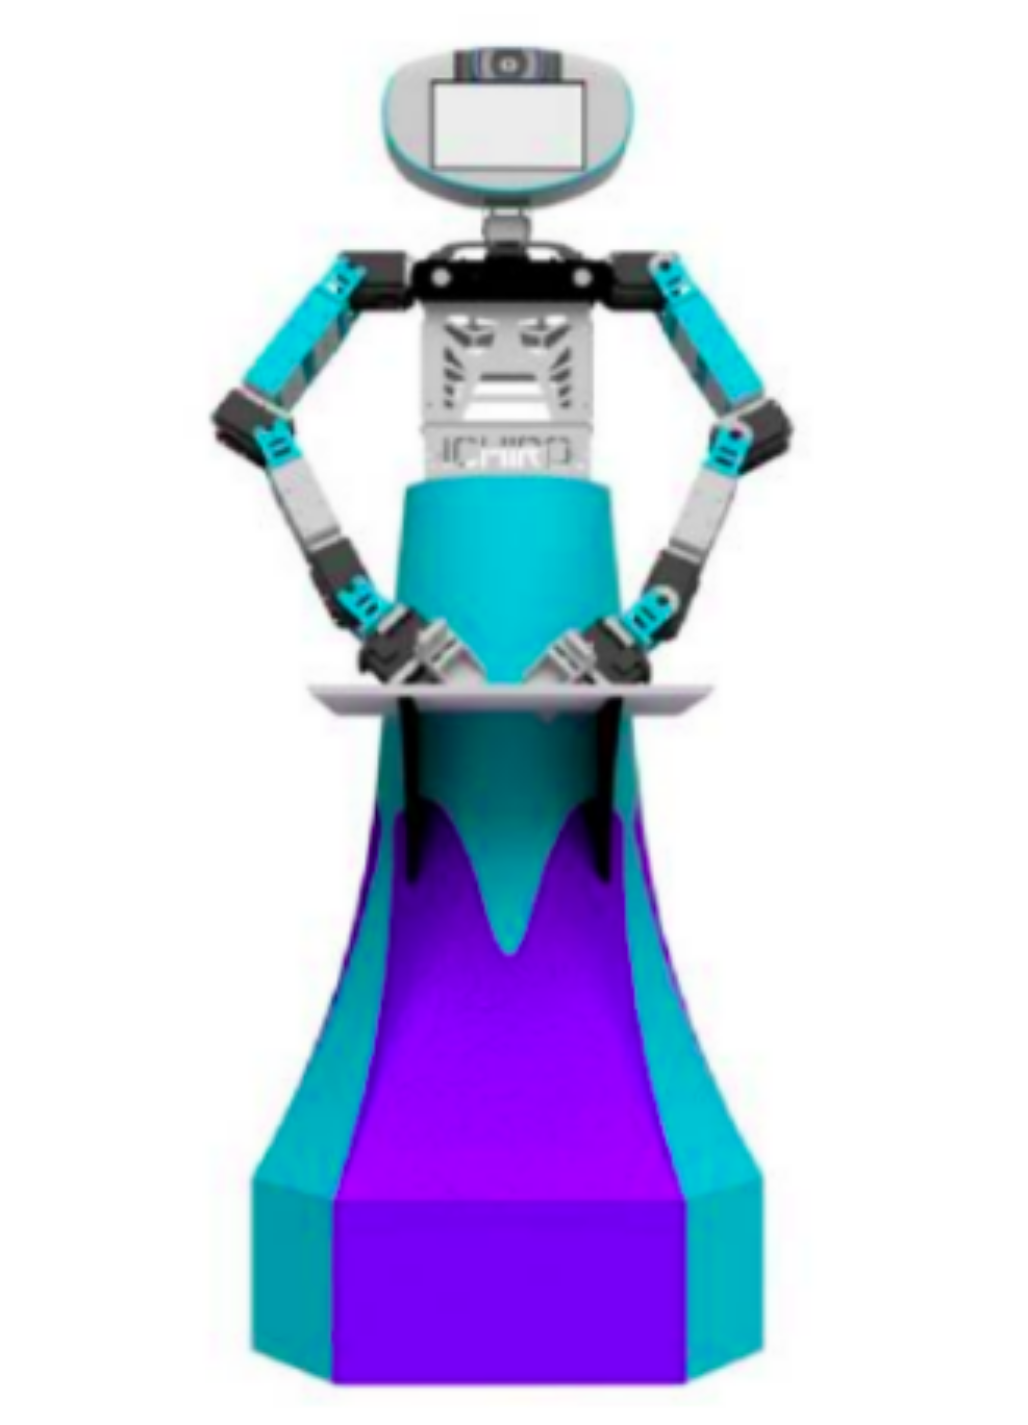
\includegraphics[scale=0.6]{gambar/desainrobot.png}
  \caption{Diagram desain robot \emph{Dienen}}
  \label{fig:desainrobot}
\end{figure}

Robot yang akan digunakan pada pada penelitian ini adalah robot \emph{Dienen} yang merupakan kelanjutan dari robot \emph{IRIS} \citep{dikairono2020}\citep{zanuar2019} dengan penambahan desain dari robot \emph{ICHIRO} \citep{muhtadin2019} di bagian atas robot.
Desain seperti ini secara umum dikenal sebagai desain \emph{mobile humanoid robot} \citep{mohamed2012}, yang merupakan desain gabungan antara robot mobile dan robot humanoid.
Seperti yang terlihat pada Gambar \ref{fig:desainrobot}, bagian bawah robot menyerupai robot mobile dengan penggerak \emph{omnidirectional wheels} yang memungkinkan pergerakan robot secara \emph{holonomic} ke segala arah\citep{oliveira2008}, sedangkan bagian atas robot menyerupai robot humanoid yang terdiri atas badan, kepala, dan lengan.
Dengan desain mobile humanoid robot ini, diharapkan pengguna bisa merasakan interaksi sosial yang lebih baik dengan robot karena memiliki bentuk mendekati manusia \citep{rossi2018} sekaligus mempermudah navigasi dari robot ke berbagai tempat.

Robot \emph{Dienen} dilengkapi dengan beberapa sensor seperti IMU (\emph{inertial measurement unit}) untuk mengetahui orientasi dari robot, \emph{rotary encoder} untuk melakukan perhitungan odometri dari robot, \emph{distance sensor} untuk mendeteksi adanya objek lain di sekitar robot, sensor kamera di kepala untuk menangkap citra, dan sensor \emph{depth camera} yang nantinya bisa digunakan untuk melakukan mapping dari ruangan.
Selain itu robot ini juga dilengkapi dengan dua lengan seperti robot manipulator yang bisa diatur pada berbagai posisi dan orientasi \citep{iqbal2012}.
Dengan adanya sensor dan aktuator ini diharapkan robot mampu melakukan tindakan \emph{assistive} secara sosial sesuai dengan data yang didapatkan dari sensor yang ada.

\subsection{Desain Kontroler Robot}

\begin{figure*} [ht]
  \centering
  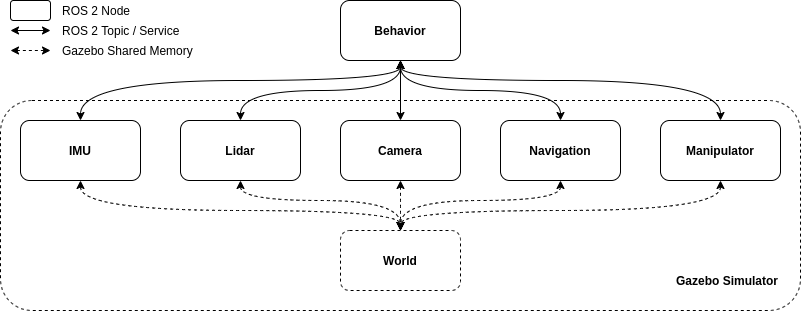
\includegraphics[scale=0.5]{gambar/kontrolerrobot.png}
  \caption{Diagram sistem dari kontroler robot}
  \label{fig:kontrolerrobot}
\end{figure*}

Kontroler robot yang digunakan untuk simulasi akan dikembangkan menggunakan ROS 2.
Kontroler tersebut akan terpisah menjadi beberapa node seperti yang terlihat pada Gambar \ref{fig:kontrolerrobot}.
Setiap node yang ada akan terhubung satu sama lain menggunakan sistem komunikasi antar proses ROS 2 yang berupa topics dan services.

Bagian utama dari kontroler robot tersebut adalah node Behavior yang berisi program yang mengatur segala tindakan robot berdasarkan data yang didapat dari sensor yang ada di simulasi.
Kemudian node Behavior tersebut akan terhubung dengan lima node lain yang merepresentasikan sensor dan aktuator yang ada pada robot.
Kelima node tersebut akan terpasang di dalam cakupan simulator Gazebo dalam bentuk plugins, sehingga mampu digunakan untuk mengakses dan memanipulasi data yang ada di simulasi menggunakan sistem \emph{shared memory} pada Gazebo \citep{gazeboplugins}.

Sistem ini dirancang secara terpisah agar node Behavior yang diujikan di lingkungan simulasi bisa langsung bekerja pada robot fisik dengan cara mengubah keseluruhan cakupan yang ada di simulator Gazebo, termasuk kelima node yang telah disebutkan sebelumnya, menjadi node yang memproses sensor dan aktuator yang ada pada robot fisik.
Dengan ini pengujian yang dilakukan di simulasi bisa langsung diterapkan ketika diujikan pada robot fisik karena tidak perlunya pembuatan ulang kontroler yang menyesuaikan sistem yang ada pada robot.

\subsection{Transfer Kontroler ke Robot Fisik}

\begin{figure*} [ht] \centering
  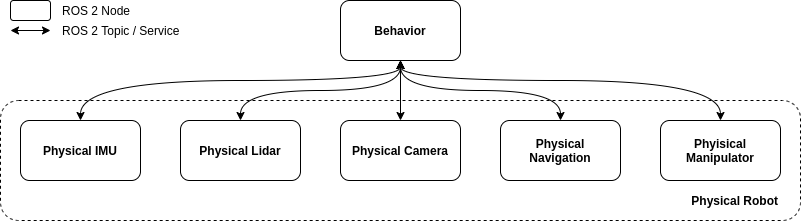
\includegraphics[scale=0.5]{gambar/transferkontroler.png}
  \caption{Diagram sistem dari kontroler robot untuk robot fisik.}
  \label{fig:transferkontroler}
\end{figure*}

Untuk memastikan kontroler robot juga bisa bekerja di luar lingkungan simulasi, pengujian juga akan dilakukan pada robot fisik dengan cara menjalankan node Behavior yang sebelumnya digunakan di lingkungan simulasi.
Seperti yang terlihat pada Gambar \ref{fig:transferkontroler}, keseluruhan cakupan yang ada di simulator Gazebo akan digantikan dengan node-node lain yang memproses sensor dan aktuator yang ada pada robot fisik.
Node-node tersebut akan terhubung dengan node Behavior menggunakan komunikasi antar proses yang ada di ROS 2.
Untuk memastikan kontroler robot dapat bekerja dengan keseluruhan sensor dan aktuator yang ada di robot fisik, maka kedua cara pengujian yang dilakukan di lingkungan simulasi sebelumnya juga akan dilakukan pada robot fisik.
Percobaan pemindahan ini dilakukan untuk memastikan bahwa pengujian yang dilakukan di lingkungan simulasi dapat digunakan untuk menggantikan pengujian yang dilakukan menggunakan robot fisik.
